La très grosse maladresse de la méthode \quote{une base à la fois} est de ne pas chercher à profiter de chaque déplacement du trou pour arranger la situation. Nous allons juste considérer cette idée pour proposer une nouvelle méthode de résolution
\footnote{
    Cette méthode a été proposée par les personnes en charge de la formation d'\quote{Informatique Débranchée} proposée par l'Académie de Grenoble le jeudi 5 janvier 2017. Voir la section \quote{Origine du jeu}.
}
qui elle aussi commence par mettre les bases en ligne de la base noire vers la rouge, et interdit tout mouvement de la base rouge à la base noire.

\begin{enumerate}
    \item On ordonne les couleurs, pour cela nous dirons que lorsque l'on va de la gauche vers la droite, on passe de couleurs froides à des couleurs chaudes.

    \item On commence par déplacer le trou vers la base rouge la plus chaude. Lors de ce déplacement, il faut déplacer à chaque fois le jeton le plus froid vers la gauche. Si les deux jetons de la base où va aller le trou sont de même chaleur, on choisit au hasard l'un des deux jetons.

    \item Une fois arrivé à la base rouge, on bouge le trou vers la base noire la plus froide. Lors de ce déplacement, ce sont les jetons les plus chauds qui migrent vers la droite. Si l'on tombe sur deux jetons de même chaleur, on applique la même tactique que ci-dessus.

    \item On continue les deux opérations $2$ et $3$ tant que toutes les bases ne sont pas complètes.
\end{enumerate}


Voici le début de l'application de cette méthode.

\medskip

\begin{multicols}{2}
    \begin{center}   % [1, 2, 3, None, 4, 1, 4, 0, 2, 3]
        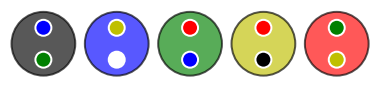
\includegraphics[scale= 0.45]{content/algo_bubble/example/000.png}

        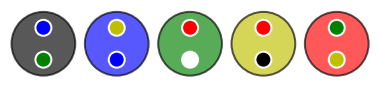
\includegraphics[scale= 0.45]{content/algo_bubble/example/001.png}

        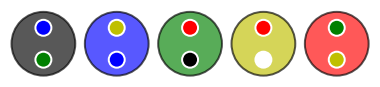
\includegraphics[scale= 0.45]{content/algo_bubble/example/002.png}

        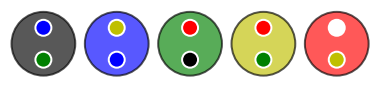
\includegraphics[scale= 0.45]{content/algo_bubble/example/003.png}

        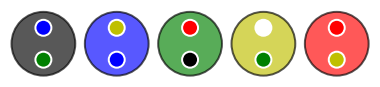
\includegraphics[scale= 0.45]{content/algo_bubble/example/004.png}

        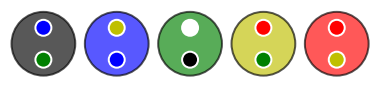
\includegraphics[scale= 0.45]{content/algo_bubble/example/005.png}

        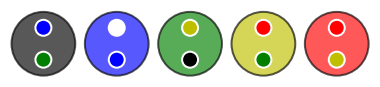
\includegraphics[scale= 0.45]{content/algo_bubble/example/006.png}

        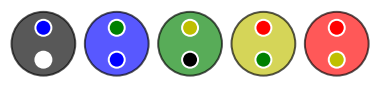
\includegraphics[scale= 0.45]{content/algo_bubble/example/007.png}
    \end{center}

    \columnbreak

    \begin{center}
        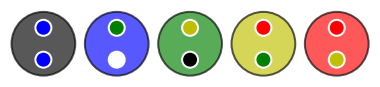
\includegraphics[scale= 0.45]{content/algo_bubble/example/008.png}

        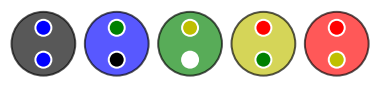
\includegraphics[scale= 0.45]{content/algo_bubble/example/009.png}

        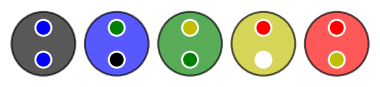
\includegraphics[scale= 0.45]{content/algo_bubble/example/010.png}

        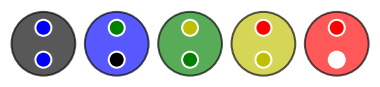
\includegraphics[scale= 0.45]{content/algo_bubble/example/011.png}

        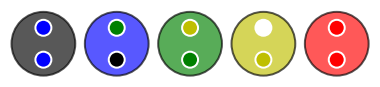
\includegraphics[scale= 0.45]{content/algo_bubble/example/012.png}

        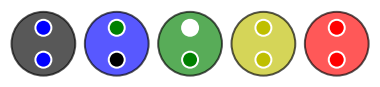
\includegraphics[scale= 0.45]{content/algo_bubble/example/013.png}

        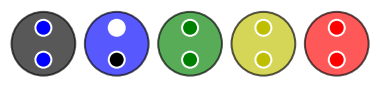
\includegraphics[scale= 0.45]{content/algo_bubble/example/014.png}

        \textbf{\vdots}

        \textbf{etc}
    \end{center}
\end{multicols}


Intuitivement, on sent bien que l'on ne va pas entrer dans une boucle infinie mais encore faut-il passer de l'intuition à une preuve irréfutable. Pour cela donnons d'abord une version plus formelle de notre nouvel algorithme de résolution (pour ordonner les couleurs nous allons les numéroter afin de simplifier les explications tout en raisonnant de façon très générale).

\bigskip

\begin{algo}
    \Data{une configuration en ligne quelconque de début de jeu}
    \Result{une configuration en ligne où tous les jetons sont rentrées dans leur base}
    \vspace{0.4em}
    \Begin{
        \vspace{0.4em}
        On numérote de $0$ à $4$ les bases de la gauche vers la droite.
        \\
        On associe chaque couleur au numéro de la base de la dite couleur.
        \\
        \vspace{0.4em}
        \tcp{d donne la direction que doit suivre le trou.}
        \tcp{\quad \textbullet{} d = 1  pour un déplacement vers la droite.}
        \tcp{\quad \textbullet{} d = -1 pour un déplacement vers la gauche.}
        $d \leftarrow 1$
        \\
        \vspace{0.4em}
        \While{la configuration contient un jeton qui n'est pas dans sa base}{
            \vspace{0.4em}
            $t$ : numéro de la base où est le trou.
            \\
            \vspace{0.4em}
            \uIf{$(d \, , t) = (1 \, , 4)$}{
                \vspace{0.4em}
                $d \leftarrow (-1)$
                \\
                \vspace{0.4em}
            }
            \uElseIf{$(d \, , t) = (-1 \, , 0)$}{
                \vspace{0.4em}
                $d \leftarrow 1$
                \\
                \vspace{0.4em}
            }
            \Else{
                \vspace{0.4em}
                \tcp{v est le numéro de la base voisine de celle du trou où l'on doit mettre ce dernier.}
                $v \leftarrow t + d$
                \\
                \vspace{0.4em}
                \uIf{d = 1}{
                    \vspace{0.4em}
                    $min$ : minimum des numéros des couleurs des jetons dans la base n°$v$.
                    \\
                    Déplacer un jeton de couleur $min$
                    de la base n°$v$ vers la base n°$t$.
                    \\
                    \vspace{0.4em}
                }
                \Else{
                    \vspace{0.4em}
                    $max$ : maximum des numéros des couleurs des jetons dans la base n°$v$.
                    \\
                    Déplacer un jeton de couleur $max$
                    de la base n°$v$ vers la base n°$t$.
                }
            }
        }
    }
\end{algo}


\bigskip

Les instructions sont clairement non ambigües. Prouvons les propriétés de \quote{finitude} et de \quote{résolution}.

\begin{proof}
    À chaque configuration $\mathscr{C}$, on associe une liste $L({\mathscr{C})}$ de nombres comme suit (des exemples visuels sont donnés un peu plus bas).

    \begin{enumerate}
        \item À chaque jeton on associe le numéro de sa couleur, et l'on considère le trou comme un jeton associé à l'entier $(-1)$.

        \item Commençons alors par considérer les jetons de la base n°0.

        \begin{enumerate}
            \item Si les deux jetons sont de la même valeur $x$, on définit la liste $L({\mathscr{C})} = [x \, , x]$ notée en utilisant des crochets. Dans une liste, l'ordre d'écriture est important et il peut y avoir des répétitions.

            \item Si les deux jetons sont de valeurs différentes $x$ et $y$, on définit la liste $L({\mathscr{C})} = [x \, , y]$ si $x < y$, et $L({\mathscr{C})} = [y \, , x]$ sinon.
        \end{enumerate}

        En résumé, $L({\mathscr{C})} = [\alpha \, , \beta]$ avec $\alpha$ et $\beta$ où sont les valeurs des jetons sur la base n°0.

        \item Ensuite on passe aux jetons de la base n°1.

        \begin{enumerate}
            \item Si les deux jetons sont de la même valeur $r$, on \quote{augmente} la liste $L({\mathscr{C})}$ en lui adjoignant à droite la liste $[r \, , r]$. Ainsi si $L({\mathscr{C})} = [x \, , y]$ à la fin de l'étape n°2, on obtient ici $L({\mathscr{C})} = [x \, , y \, , r \, , r]$.

            \item Si les deux jetons sont de valeurs différentes $r$ et $s$, à la liste $L({\mathscr{C})}$ on adjoint à droite soit la liste $[r \, , s]$ si $r < s$, soit $[s \, , r]$ sinon. Ainsi si $L({\mathscr{C})} = [x \, , y]$ à la fin de l'étape n°2, on obtient ici $L({\mathscr{C})} = [x \, , y \, , r \, , s]$ ou $L({\mathscr{C})} = [x \, , y \, , s \, , r]$ suivant les cas.
        \end{enumerate}

        \item On fait de même avec la base n°2, puis la n°3, \dots \textit{etc.}
    \end{enumerate}

    En termes plus courants, dans chaque base on ordonne les jetons de la valeur la plus petite à la valeur la plus grande, puis on \quote{accole dans une liste} les couples \quote{ordonnés} ainsi formés. Voici des exemples.

    \vspace{-0.4em}
    \begin{center}   % [2, 2, 3, None, 3, 1, 4, 0, 4, 1]
        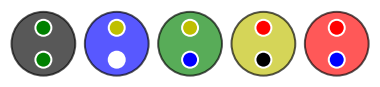
\includegraphics[scale= 0.45]{content/algo_bubble/modelization/example_a.png}

        [{\color{black} 2 , 2} , {\color{blue} $-1$ , 3} , {\color{ForestGreen} 1 , 3} , {\color{Goldenrod} 0 , 4} , {\color{red} 1 , 4}]


        \medskip     % [4, 2, 3, 0, 2, 3, 1, 4, 1, None]

        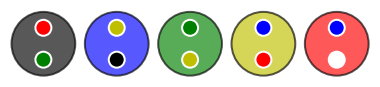
\includegraphics[scale= 0.45]{content/algo_bubble/modelization/example_b.png}

        [{\color{black} 2 , 4} , {\color{blue} 0 , 3} , {\color{ForestGreen} 2 , 3} , {\color{Goldenrod} 1 , 4} , {\color{red} $-1$ , 1}]
    \end{center}

    Les listes de nombres de même taille sont comparables comme le sont les mots d'un dictionnaire, on parle d'ordre lexicographique. Par exemple, nous avons :

    \medskip

    \begin{itemize}
        \item[\textbullet] $[\text{\color{red} \textbf{2} , \textbf{2} , \textbf{3}} \, , 1 \, , 3 \, , 0 \, , 4 \, , 1 \, , 4] > [\text{\color{red} \textbf{2} , \textbf{2} , \textbf{1}} \, , 3 \, , 0 \, , 4 \, , 1 \, , 3 \, , 4]$
        en comparant le $3$ et le $1$ aux troisièmes positions qui sont les premières valeurs à être différentes (par contre peu importe ce qu'il y a aux positions suivantes).

        \medskip

        \item[\textbullet] $[\text{\color{red} \textbf{1}} \, , 2 \, , 2 \, , 3 \, , 3 \, , 0 \, , 4 \, , 1 \, , 4] < [\text{\color{red} \textbf{2}} \, , 2 \, , 3 \, , 1 \, , 3 \, , 0 \, , 4 \, , 1 \, , 4]$
        en comparant le $1$ et le $2$ aux premières positions (sans se soucier des nombres qui suivent).
    \end{itemize}


    \medskip

    Nous n'allons pas comparer les deux listes $L(\mathscr{C}_1)$ et $L(\mathscr{C}_2)$ associées à deux configurations $\mathscr{C}_1$ et $\mathscr{C}_2$. Nous allons considérer à la place les sous-listes $SL(\mathscr{C}_1)$ et $SL(\mathscr{C}_2)$ obtenues en retirant le seul $(-1)$ présent dans les listes $L(\mathscr{C}_1)$ et $L(\mathscr{C}_2)$ respectivement (bien noter que les listes comparées via l'ordre lexicographique sont celles sans $(-1)$ la valeur du trou).


    \medskip

    Nous voilà armés pour faire notre démonstration sans encombre (mais pas sans réflexion).


    \medskip

    \textit{Fait n°1 : si le trou n'est pas dans la base n°0 alors les mouvements indiqués par l'algorithme amène le trou dans la base n°0.}


    \medskip

    C'est évident à condition d'avoir bien noté que pour la configuration gagnante, le trou est dans la base n°0.


    \medskip

    \textit{Fait n°2 : la configuration gagnante est la seule telle que le trou soit dans la base n°0 et telle que sa sous-liste soit minimale (c'est à dire qu'elle est inférieure ou égale à toutes les listes $SL(\mathscr{C})$ possibles).}


    \medskip

    Soit $\mathscr{G}$ la configuration gagnante. Il est clair que
    $SL(\mathscr{G}) = \text{[0 , 1 , 1 , 2 , 2 , \dots{} ]}$
    et que le trou est dans la base n°0.


    \medskip

    Soit $\mathscr{C}$ une configuration non gagnante. Si $SL(\mathscr{C}) \neq SL(\mathscr{G})$, il est évident que $SL(\mathscr{C}) > SL(\mathscr{G})$. Sinon si $SL(\mathscr{C}) = SL(\mathscr{G})$ c'est que le trou n'est pas dans la base n°0.


    \medskip

    \textit{Fait n°3 : lorsque l'un des mouvements demandés par l'algorithme est effectué, on passe d'une configuration $\mathscr{C}_1$ à une configuration $\mathscr{C}_2$. On a alors la relation : $SL(\mathscr{C}_2) \leqslant SL(\mathscr{C}_1)$.}


    \medskip

    Considérons le cas où le trou se déplace vers la droite.
    Notons $L(\mathscr{C}_1) = [ \text{\ \dots{} , $-1$ , $x$ , $y$ , $z$ , \dots{} \ } ]$ où les points de suspension indiquent des éventuelles paires de valeurs.
    En particulier, $(-1)$ et $x$ sont les valeurs du trou et du jeton partageant la même base, tandis que $y$ et $z$ sont celles de deux autres jetons dans la base voisine à droite (notons que forcément $y \leqslant z$). Nous avons deux situations.

    \begin{enumerate}
        \item \textbf{Cas 1 :} $x \leqslant y$.

        Dans ce cas, $L(\mathscr{C}_2) = [ \text{\ \dots{} , $x$ , $y$ , $-1$ , $z$ , \dots{} \ } ]$ d'où $SL(\mathscr{C}_2) = SL(\mathscr{C}_1)$.

        \item \textbf{Cas 2 :} $y < x$.

        Dans ce cas, $L(\mathscr{C}_2) = [ \text{\ \dots{} , $y$ , $x$ , $-1$ , $z$ , \dots{} \ } ]$ d'où $SL(\mathscr{C}_2) < SL(\mathscr{C}_1)$.
        \end{enumerate}

    Le cas d'un déplacement vers la gauche se traite de façon analogue.


    \medskip

    \textit{Fait n°4 : si $\mathscr{C}$ est une configuration telle que $SL(\mathscr{C})$ ne soit pas minimale, l'algorithme fera apparaître à un moment ou à un autre une configuration $\mathscr{C}^\prime$ telle que $SL(\mathscr{C}^\prime) < SL(\mathscr{C})$ (en fait, le dit moment arrivera avant un éventuel aller-retour \quote{complet} du trou depuis sa base dans la configuration $\mathscr{C}$).}


    \medskip

    Comme $SL(\mathscr{C})$ n'est pas minimale, il existe au moins deux valeurs $x$ et $y$ telles que $x > y$ avec $y$ situé après $x$ dans $SL(\mathscr{C})$ lorsqu'on lit cette liste de gauche à droite.
    La condition $x > y$ implique que $x$ et $y$ ne sont pas dans la même base. Nous avons : $L(\mathscr{C}) = [ \text{\ \dots{} , $x$ , \dots{} , $y$ , \dots{} \ } ]$ où les points de suspension indiquent d'éventuelles valeurs.


    \medskip

    Parmi tous les $y$ possibles, on choisit celui qui est le plus à gauche possible dans $SL(\mathscr{C})$, c'est à dire celui qui est le plus prêt de $x$ (dans ce cas, $y$ est la plus petite valeur de sa base).
    Avec ce choix, les valeurs éventuelles $w$ entre $x$ et $y$ dans $SL(\mathscr{C})$ vérifient toutes $y < x \leqslant w$. Ceci permet donc de choisir $x$ et $y$ voisins dans $SL(\mathscr{C})$ (avec des bases associés voisines différentes).
    Avec ce nouveau choix, $L(\mathscr{C}) = [ \text{\ \dots{} , $g$ , $x$ , $y$ , $d$ , \dots{} \ } ]$ où les points de suspension indiquent des éventuelles paires de valeurs. Notons que seul $g$ peut être égal à $(-1)$.
    Désignons par $\mathcal{B}_x$ et $\mathcal{B}_y$ les basses associées aux valeurs $x$ et $y$.


    \medskip

    Rappelons que tant que $SL(\mathscr{C})$ n'est pas minimale, la configuration $\mathscr{C}$ n'est pas une configuration gagnante et donc le trou se balade. Nous avons alors les situations suivantes.

    \begin{enumerate}
        \item \textbf{Cas 1 :} $g = -1$

        Si l'algorithme est dans une phase de déplacement vers la droite, alors comme dans la preuve du fait n°3, voir son cas 2, nous savons que la configuration suivante $\mathscr{C}^\prime$ vérifie $SL(\mathscr{C}^\prime) < SL(\mathscr{C})$ ce qui prouve ici le fait n°4.

        Sinon le trou va aller vers la base n°0. Si lors de ces déplacements, l'une des configurations $\mathscr{C}^\prime$ vérifie $SL(\mathscr{C}^\prime) < SL(\mathscr{C})$ alors le fait n°4 sera validé. Sinon le trou reviendra en direction de la base $\mathcal{B}_x$. Si lors de ces déplacements, l'une des configurations $\mathscr{C}^\prime$ vérifie $SL(\mathscr{C}^\prime) < SL(\mathscr{C})$ alors le fait n°4 sera validé. Sinon nous nous retrouvons dans le sous-cas traité ci-dessus où l'on avait un déplacement du trou vers la droite avec $g = -1$, et de nouveau nous obtenons le résultat souhaité.

        \item \textbf{Cas 2 :} $g \neq -1$ et le trou est à gauche de la base $\mathcal{B}_x$.

        Si l'algorithme est dans une phase de déplacement vers la droite, alors le trou va prendre la place de $g$ et l'on retombe dans le cas 1. Si le déplacement se fait vers la gauche, on peut appliquer exactement le même raisonnement que dans le deuxième sous-cas du cas 1 traité ci-dessus.

        \item \textbf{Cas 3 :} $g \neq -1$ et le trou est à droite de la base $\mathcal{B}_y$.

        L'algorithme va amener le trou dans la base voisine de $\mathcal{B}_y$ de sorte que l'on ait une configuration $\mathscr{C}^\prime$ telle que $L(\mathscr{C}^\prime) = [ \text{\ \dots{} , $g$ , $x$ , $y$ , $d$ , $-1$ , $\alpha$ , \dots{} \ } ]$ avec $SL(\mathscr{C}^\prime)$ non minimal.

        Si lors de ces déplacements une configuration $\mathscr{C}^{\prime\prime}$ vérifie $SL(\mathscr{C}^{\prime\prime}) < SL(\mathscr{C})$, le fait n°4 est bien entendu vérifié.
        Sinon $L(\mathscr{C}^\prime)$ devient $[ \text{\ \dots{} , $g$ , $x$ , $-1$ , $y$ , $?$ , $?$ , \dots{} \ } ]$, puis $[ \text{\ \dots{} , $-1$ , $g$ , {\color{red} $y$ , $x$} , $?$ , $?$ , \dots{} \ } ]$ où l'on utilisé le fait que $y < x$. Pour cette dernière liste, la configuration $\mathscr{C}^{\prime\prime\prime}$ vérifie $SL(\mathscr{C}^{\prime\prime\prime}) < SL(\mathscr{C})$ et c'est gagné !
    \end{enumerate}


    \medskip

    \textit{Finitude et résolution} : le fait n°1 nous permet de considérer le 1er moment où le trou est dans la base n°0.
    Si nous avons une configuration $\mathscr{C}$ gagnante, nous nous arrêtons comme demandé et il n'y a rien à prouver.


    \medskip

    Sinon la configuration $\mathscr{C}$  est telle que $SL(\mathscr{C})$ ne soit pas minimale d'après le fait n°2.
    Grâce au fait n°4, nous savons que nous arriverons ensuite à une configuration $\mathscr{C}^\prime$ telle que $SL(\mathscr{C}^\prime) < SL(\mathscr{C})$.
    Dès lors les faits n°3 et n°1 nous permettent d'affirmer que le trou va se retrouver dans base n°0 pour une configuration $\mathscr{C}^{\prime\prime}$ telle que $SL(\mathscr{C}^{\prime\prime}) \leqslant SL(\mathscr{C}^\prime) < SL(\mathscr{C})$.


    \medskip

    En résumé, si le trou se retrouve dans la base n°0 pour une configuration $\mathscr{C}$ non gagnante, alors l'algorithme nous fera déplacer le trou jusqu'à le faire arriver de nouveau dans la base n°0 pour une nouvelle configuration $\mathscr{C}^{\prime\prime}$ telle que $SL(\mathscr{C}^{\prime\prime}) < SL(\mathscr{C})$.


    \medskip

    Pour conclure, il suffit de noter que le nombre de listes $SL(\mathscr{C})$ est fini.
    Dès lors il est impossible d'avoir une suite strictement décroissante de listes du type $SL(\mathscr{C})$.
    Ceci signifie que l'algorithme va en un nombre fini d'étapes amener le trou dans la base n°0 pour une configuration gagnante.
\end{proof}


\paragraph{Remarque :} \hspace{-1em} la démonstration s'adapte sans problème à un nombre quelconque $n \geqslant 2$ de bases.
